    \documentclass{article}
% The LaTeX macro language is complicated, so we have inserted
% lots of documenting comments into the file.  Comments start
% with `%' and continue to the end of the line.  In Overleaf's
% window, they are colored green
%
% Comments prefixed with `Student:' are relevant to students.
% Skip anything else you don't understand, or ask me.
%
% set font encoding for PDFLaTeX or XeLaTeX
\usepackage{ifxetex}
\ifxetex
  \usepackage{fontspec}
\else
  \usepackage[T1]{fontenc}
  \usepackage[utf8]{inputenc}
  \usepackage{lmodern}
\fi

% Student: These lines describe some document metadata.
\title{Problem Set 8}
\author{%
% Student: change the next line to your name!
    Name
\\  MATH-UA 120 Discrete Mathematics
}
\date{due Dec 8, 2023}


\usepackage[headings=runin-fixed-nr]{exsheets}
% These make enumerates within questions start at the second ("(a)") level, rather than the first ("1.") level.
\makeatletter
    \newcommand{\stepenumdepth}{\advance\@enumdepth\@ne}
\makeatother
\SetupExSheets{
    question/pre-body-hook=\stepenumdepth,
    solution/pre-body-hook=\stepenumdepth,
}
\DeclareInstance{exsheets-heading}{runin-nn-np}{default}{
    runin = true,
    title-post-code = .\space,
    join = {
        main[r,vc]title[l,vc](0pt,0pt);
    }
}
\newif\ifshowsolutions
% Student: replace `false' with `true' to typeset your solutions.
% Otherwise they are ignored!
\showsolutionstrue
\ifshowsolutions
    \SetupExSheets{
        question/pre-hook=\itshape,
        solution/headings=runin-nn-np,
        solution/print=true,
        solution/name=Answer
    }%
    \makeatletter%
    \pretocmd{\@title}{Answers to }%
    \makeatother%
\else
    \SetupExSheets{solution/print=false}
\fi

% Bug workaround: http://tex.stackexchange.com/a/146536/1402
%\newenvironment{exercise}{}{}
\RenewQuSolPair{question}{solution}
%\let\answer\solution
%\let\endanswer\endsolution
\usepackage{manfnt}
\newcommand{\danger}{\marginpar[\hfill\dbend]{\dbend\hfill}}

% We are creating a command for some common commands.
\newcommand{\Z}{\mathbb{Z}}
\newcommand{\N}{\mathbb{N}}
\newcommand{\modulo}{\text{mod }}
\newcommand{\divisor}{\text{ div }}

% This package is for specifying graphics.  It's amazing.
% Manual at http://texdoc.net/texmf-dist/doc/generic/pgf/pgfmanual.pdf
\usepackage{tikz}
\tikzstyle{vertex}=[circle,draw,fill=none,inner sep=0pt,outer sep=0pt, minimum width=1ex]
\tikzstyle{edge}=[draw,thick]
\usepackage{multirow, multicol}
\usepackage{amsmath, amsthm, amssymb}
\usepackage{amsfonts}
\usepackage{siunitx}
\DeclareSIUnit\pound{lb}
\usepackage{hyperref}
\newtheorem*{theorem}{Theorem}
\theoremstyle{definition}
\newtheorem*{definition}{Definition}
\newenvironment{note}{\noindent\emph{Note}.}{}
% This is the beginning of the part of the file that describes
% the text of the document.
% That's why it says `\begin{document}' below. :-)
\begin{document}
\maketitle



These are to be written up and turned in to Gradescope.\\



\ifshowsolutions
    \SetupExSheets{solution/print=true}
\else
    \danger
 \underline{ \LaTeX  Instructions:}  You can view the source (\texttt{.tex}) file to get some more examples of \LaTeX{} code.  I have commented the source file in places where new \LaTeX{} constructions are used.
  
  Remember to change \verb|\showsolutionsfalse| to \verb|\showsolutionstrue|
    in the document's preamble 
    (between \verb|\documentclass{article}| and \verb|\begin{document}|)
\fi

\section*{Assigned Problems}



\begin{question}
    \begin{enumerate}
        \item Find $d = \gcd(29341,1739)$, and integers $x$ and $y$ such that $29341x + 1739y = d$.
        \item Prove that 7 cannot be expressed as an integral linear combination of 29341 and 1739.
    \end{enumerate}
\end{question}
% Student: put your answer between the next two lines.
\begin{solution}
    \begin{enumerate}
        \item By the Euclidean algorithm:
            \begin{align*}
                29341 &= 16 \times 1739 + 1517
                 &\implies 1517 &= 29341 - 16 \times 1739 \\
                 1739 &= 1 \times 1517 + 222
                 &\implies  222 &= 1739 - 1 \times 1517 \\
                 1517 &= 6 \times 222 + 185
                 &\implies  185 &= 1517 - 6 \times 222 \\
                  222 &= 1 \times 185 + 37
                  &\implies  37 &= 222 - 1 \times 185 \\
                  185 &= 5 \times 37 + 0
            \end{align*}
            So $\gcd(1739,29341) = 37$.  Working backwards,
            \begin{align*}
                37 &= 222 - 1 \times 185 \\
                   &= 222 - 1 \times (1517 - 6 \times 222)
                    = 7 \times 222 - 1 \times 1517 \\
                   &= 7 \times (1739 - 1 \times 1517) - 1 \times 1517
                    = 7 \times 1739 - 8 \times 1517 \\
                   &= 7 \times 1739 - 8 \times (29341 - 16 \times 1739)
                    = 135 \times 1739 - 8 \times 29341
            \end{align*}
            So $a=135$ and $b=-8$.
        \item By Theorem 36.6, the greatest common divisor is the smallest positive integer that can be expressed as an integral linear combination. Since $\gcd(1739,29341) = 37$, then 37 is the smallest positive integer that can be expressed as $1739x + 29341y$ for some integers $x, y$. Therefore, 7 cannot be expressed as an integral linear combination of 29341 and1739.
    \end{enumerate}

{\color{red} Rubric:
\begin{itemize}
\item 5P each
\end{itemize}}
\end{solution}


\begin{question}
    \begin{enumerate}
        \item Disprove: There exist integers $a$ and $b$ such that $a+b=100$ and $\gcd(a, b)=8$.
        \item Prove: There exist infinitely many pairs of integers $(a,b)$ such that $a+b=87$ and $\gcd(a, b)=3$.
    \end{enumerate}
\end{question}
% Student: put your answer between the next two lines.
\begin{solution}
\begin{enumerate}
    \item If $\gcd(a, b)=8$, then there exists $x, y\in \Z$ such that $a=8x$ and $b=8y$. If $100=a+b$, then $100=8x+8y=8(x+y)$. Then $8\mid 100$, but 8 does not divide 100.
    \item Let $n\in \Z$ such that $29\nmid n$. Choose $a=3n$ and $b=3(29-n)$. Observe that $a+b = 3n + 3(29-n) = 3n + 87-3n = 87$. Note that $3\mid a$ and $3\mid b$. We will prove $\gcd(a, b)=3$.
    \begin{proof}
    For the sake of contradiction, assume there exists $d\in \Z$ such that $d\mid a$ and $d\mid b$, and $d>3$. Since $a+b=87$, $d\mid 87$. All the factors of 87 are 1, 3, 29, and 87. Since $d>3$, $d=29$ or $d=87$. 
    \begin{itemize}
    \item If $d=29$, then $29\mid a$. Meaning, $29\mid 3n \implies 29\mid n$. Contradiction!
    \item If $d=87$, then $87\mid a$. Then there exists $x\in \Z$ such that $3n=87x\implies n=29x\implies 29\mid n$. Contradiction!
    \end{itemize}
    \end{proof}

\end{enumerate}

{\color{red} Rubric:
\begin{itemize}
\item 5P each
\end{itemize}}
\end{solution}

\begin{question}
    \begin{enumerate}
        \item Let $a, b, c\in \Z$ such that $a$ and $b$ are relatively prime. Prove that if $a\mid c$ and $b\mid c$, then $(ab)\mid c$.
        \item Explain why part (a) is false if $a$ and $b$ are not relatively prime.
    \end{enumerate}
\end{question}
% Student: put your answer between the next two lines.
\begin{solution}
\begin{enumerate}
    \item Let $a, b, c\in \Z$ such that $a$ and $b$ are relatively prime. Then there exist $x, y\in \Z$ such that $1=ax+by \implies c = acx+bcy$. Suppose $a\mid c$ and $b\mid c$. Then there exist $m, n\in \Z$ such that $c=an$ and $c=bn$. Observe
    \begin{align*}
    c &= acx+bcy \\
    & = a(bn)x+b(an)y\\
    & = ab(nx+by).
    \end{align*}
    Then $(ab)\mid c$.
    \item Let $a=4$, $b=8$, and $c=16$. Note $\gcd(a, b)=4$, so $a$ and $b$ are not relatively prime. We have that $4\mid 16$ and $8\mid 16$, but $(4\cdot 8)\nmid 16$.

\end{enumerate}

{\color{red} Rubric:
\begin{itemize}
\item 5P each
\end{itemize}}
\end{solution}

\begin{question} 
 Consider the following graph $G$.
     \begin{center}
    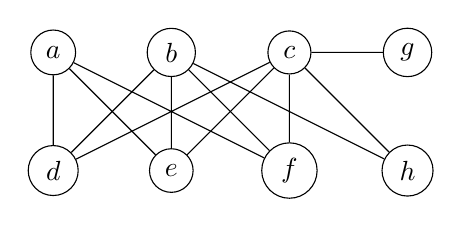
\begin{tikzpicture}[
        every node/.append style={draw,circle}
    ]
        \node (A) at (-1.5, 0) {$a$};
        \node (B) at (0, 0)    {$b$};
        \node (C) at (1.5, 0)  {$c$};
        \node (D) at (-1.5, -1.5) {$d$};
        \node (E) at (0, -1.5)   {$e$};
        \node (F) at (1.5, -1.5) {$f$};
        \node (G) at (3, 0)   {$g$};
        \node (H) at (3, -1.5) {$h$};
        \draw (A) -- (D) -- (C) -- (F) -- (A);
        \draw (A) -- (E) -- (C);
        \draw (D) -- (B) -- (F);
        \draw (G) -- (C) -- (H) -- (B) -- (E);
    \end{tikzpicture}
    \end{center}
    
\begin{enumerate}
	\item Write out the ordered pair $G=(V, E)$.
	\item What is the order of $G$?
	\item What is the size of $G$?
	\item What is $N(b)$?
	\item What is $d_G(c)$?
	\item What is $\Delta(G)$?
	\item What is $\delta(G)$?
	\item What elements are the vertex $a$ adjacent to?
	\item What elements are the vertex $f$ incident with?
	\item Is $G$ regular? Briefly explain why or why not.
	\end{enumerate}
\end{question}
% Student: put your answer between the next two lines.
\begin{solution}
\begin{enumerate}
	\item \begin{multline*}
	G=(\{a, b, c, d, e, f, g, h\}, \\ \{\{a, d\}, \{a, e\}, \{a, f\}, \{b, d\}, \{b, e\}, \{b, f\}, \{b, h\}, \{c, d\}, \{c, e\}, \{c, f\}, \{c, g\}, \{c, h\}\})
	\end{multline*}
	\item The order of $G$ is $|V|=8$.
	\item The size of $G$ is $|E|=12$.
	\item $N(b) = \{d, e, f, h\}$
	\item $d_G(c)=5$
	\item $\Delta(G)=5$
	\item $\delta(G)=1$
	\item The elements that are adjacent to vertex $a$ are vertices $d, e,$ and $f$.
	\item The elements that are incident with vertex $f$ are edges $\{a, f\}, \{b, f\},$ and $\{c, f\}$.
	\item $G$ is not a regular graph because not all vertices have the same degree.
\end{enumerate}

{\color{red} Rubric:
\begin{itemize}
\item 1P each part
\end{itemize}}
\end{solution}

\begin{question}
     Let $G=(V,E)$ be a graph. Prove by induction: 
\begin{quote}
The sum of the degrees of the vertices in $G$ is twice the number of edges.
\end{quote}	
\end{question}
% Student: put your answer between the next two lines.
\begin{solution}
Let $G=(V,E)$ be a graph and $d$ be the sum of the degree of all the vertices of $G$. We will prove $d=2|E|$ by induction.
\begin{description}
\item[Basis:] Consider $|E|=0$. If there are no edges, then the degree of all vertices must be zero. Then $d=0$ and $2|E|=0$. Hence the statement is true for $|E|=0$.
\item[Inductive Hypothesis:] Consider $|E|=n$ for $n\in \N$. Assume that $d=2n$.
\item[Inductive Step:] Consider a graph $G=(V,E)$ with $|E|=n+1$. Let $e\in E$. If we remove the edge $e$ from the graph G, then we have the graph $G'=G-e$. Graph $G'$ has $n$ edges; hence, the sum of the degree of the vertices of $G'$ is $2n$. Since $e$ cannot be a loop, it must have two distinct endpoints. Then exactly two vertices in $G'$ has one degree less than their degree in $G$. Then the sum of the degrees of the vertices of $G'$ is two less than the sum of the degrees of the vertices of $G$. So the sum of the degrees of the vertices of $G$ is $2n+2=2(n+1)$.
Therefore, by the principal of mathematical induction, the statement is true.
\end{description}

{\color{red} Rubric:
\begin{itemize}
\item RVF and \LaTeX
\end{itemize}}
\end{solution}









\end{document}

